% !TEX root = ../thesis-example.tex
%
\chapter{Représentation visuelle}
\label{ch:visual_representation}

\cleanchapterquote{Ces petits morceaux d’espace visuels, dont la connexion n’est pas donnée d’avance, par quoi voulez vous qu’ils soient connectés, sinon par la main.}{Gilles Deleuze}{in: \textit{Qu'est ce que l'acte de création?}}


%%%%%%%%%%%%%%%%%%%%%%%%%%%%%%%%%%%%%%%%%
\section{le cockpit du musicien?}
\label{sec:visual_representation:sec1}

%%%%%%%%%%%%%%%%%%%%%%%%%%%%%%%%%%%%%%%%%
\section{Guides, carte, fretting}

%%%%%%%%%%%%%%%%%%%%%%%%%%%%%%%%%%%%%%%%%
\section{représentation de l'objet/processus virtuel}

%%%%%%%%%%%%%%%%%%%%%%%%%%%%%%%%%%%%%%%%%
\section{intégration de la partition dans l'interface}

%%%%%%%%%%%%%%%%%%%%%%%%%%%%%%%%%%%%%%%%%
\section{aspects esthétiques / instruments visuels}

%%%%%%%%%%%%%%%%%%%%%%%%%%%%%%%%%%%%%%%%%
\section{La librairie mp.TUI pour Max}

La bibliothèque mp.TUI est construite sur le protocole MP. Elle fournit un cadre basé sur les logiques de patch de Max pour créer de nouveaux composants d'interface utilisateur multitouch dans un contexte OpenGL et surmonter certaines limitations de l'interface graphique native de l'environnement de patching de Max. Par exemple, les interfaces graphiques sont généralement orientées sur une disposition horizontale/verticale avec une orientation de lecture du haut vers le bas alors qu'on peut souhaiter avoir plusieurs orientations, comme dans la situation présentée sur la figure 3. La superposition de divers composants peut nécessiter des couleurs et des transparents personnalisés, et l'on peut souhaiter inclure des interfaces visuelles plus complexes que les curseurs et les boutons, par exemple des particules, des vidéos, des modèles 3d, des shaders (figure 5), etc.

La possibilité de concevoir des objets audiovisuels en Max en étroite relation avec la programmation de l'interaction entre le geste, l'audio et le visuel permet de les intégrer dans des scénarios dynamiques personnalisés : histoires narratives pour des ateliers éducatifs avec des enfants, scénarios réactifs, visualisations personnalisées pour les malvoyants, expositions muséographiques avec chartes graphiques spécifiques, adaptation réactive aux formats d'écran, graphismes expérimentaux pour l'esthétique des performances artistiques live, etc.

%-------------------------- Figure : mp.TUI ----------------------------------
\begin{figure}[htb]
	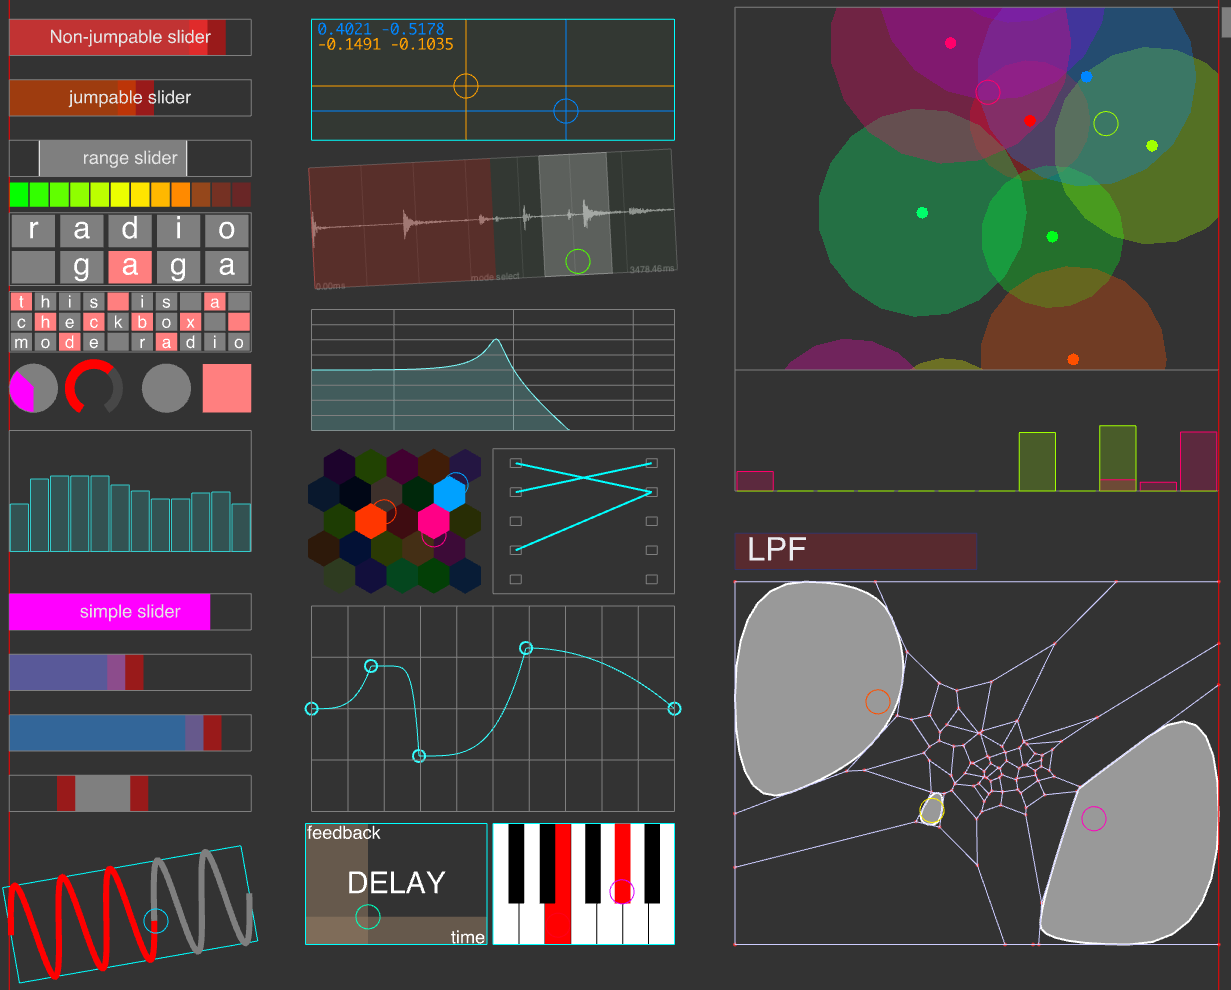
\includegraphics[width=\textwidth]{gfx/mpTUI/mp-TUI-preview.png}
	\caption{Aperçu de quelques composants graphiques de la librairie mp.TUI}
	\label{fig:visual_representation:mp.TUI}
\end{figure}

\begin{figure}
	\centering
	\begin{minipage}{.5\textwidth}
		%\centering
		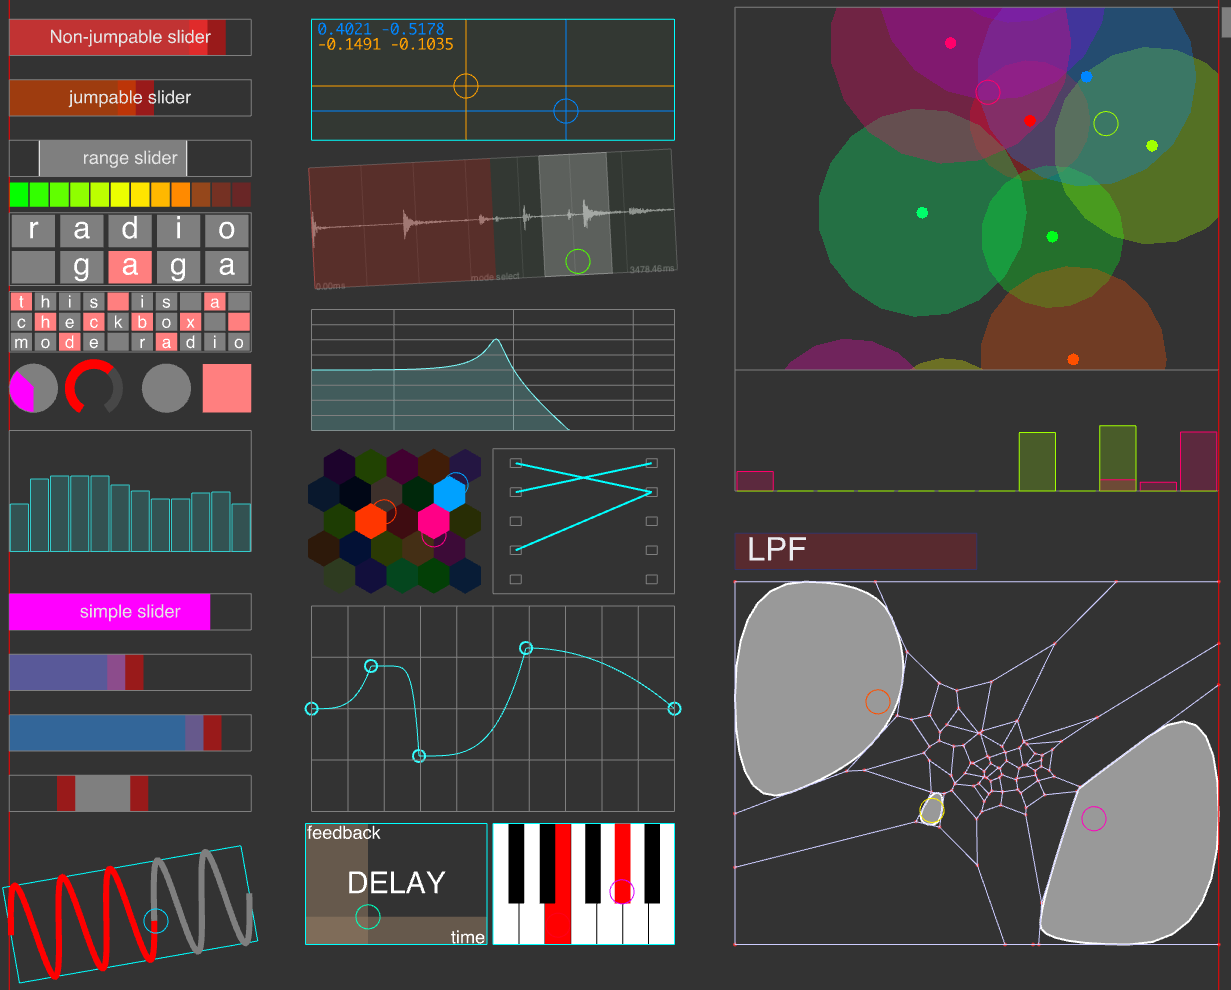
\includegraphics[width=.98\linewidth]{gfx/mpTUI/mp-TUI-preview.png}
		\captionof{figure}{Exemples de composants}	
		\label{fig:visual_representation:overview}
	\end{minipage}%
	\begin{minipage}{.5\textwidth}
		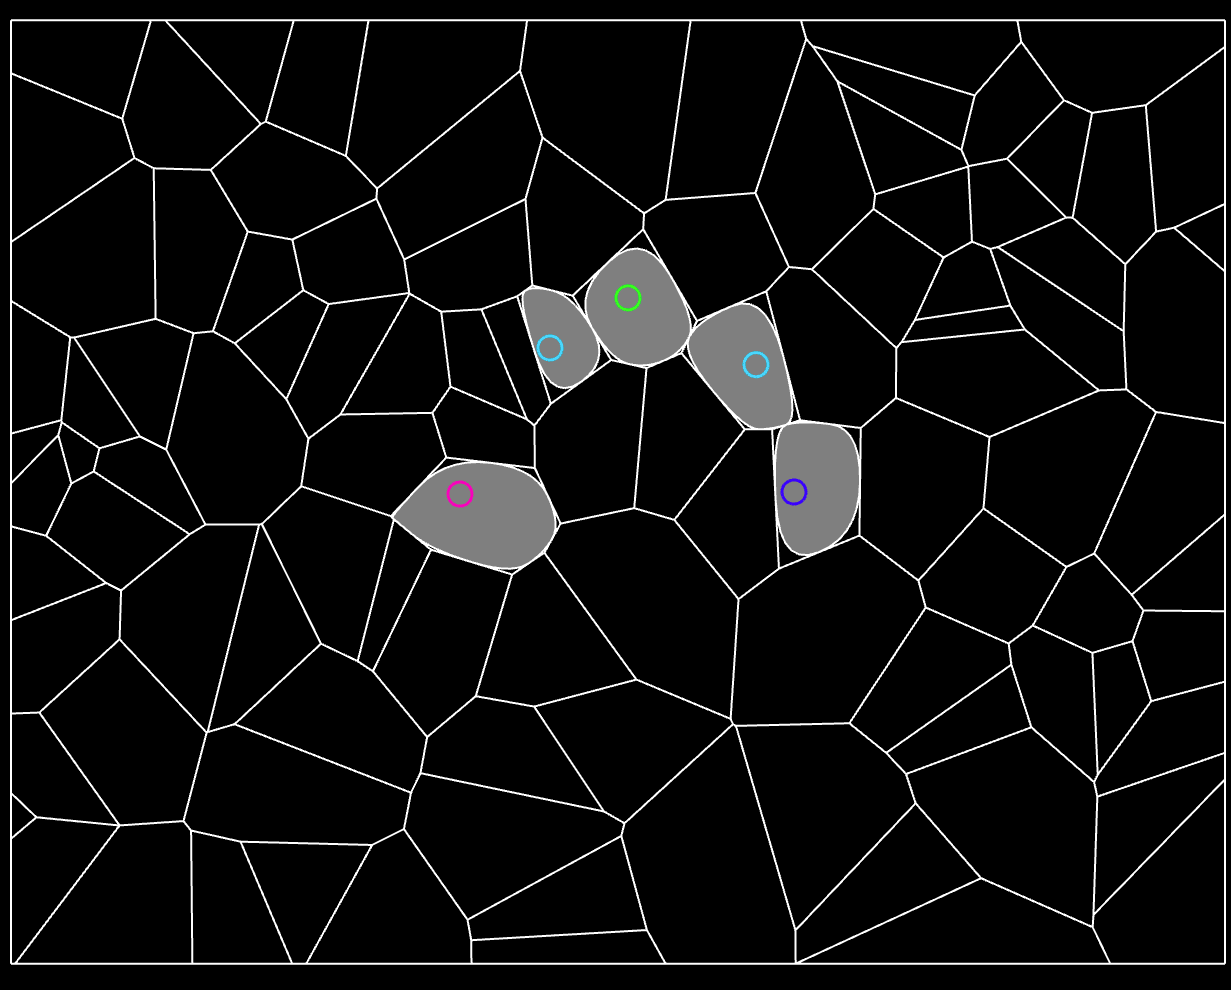
\includegraphics[width=.98\linewidth]{gfx/mpTUI/mp-TUI-voronoi.png}
		\captionof{figure}{Modèle de Voronoi}
		\label{fig:visual_representation:voronoi}
	\end{minipage}
\end{figure}

\blindtext
\blindtext

\blindtext

%%%%%%%%%%%%%%%%%%%%%%%%%%%%%%%%%%%%%%%%%
\section*{miscellanées (temporaire à supprimer)}
citations :

The  keyboards  were  always  there...  for  some  reason  or  other  it  looks  good  if  you’re playing a keyboard. People understand then you’re making music.” Robert Moog in Trevor Pinch, “Why You Go to a Piano Store to Buy a Synthesizer: Path Dependence and the Social Construction of Technology,” in Path Dependence and Creation



\begin{quote}
Visual language is one of the oldest forms of knowledge representation and predates conventional written language by almost 25,000 years
\end{quote}
\cite{tufte_visual_2001}

\cite{moody_physics_2009}


\begin{quotation}
If you ask the man on the stree "What's a synthesizer?" He will reply "A synthesizer is a keyboard instrument"... If you go in a retail store ad say I want to see some electronic instruments, they'll send you to the keyboard department, because a synthesizer is a keyboard instrument by default. — Don Buchla, synthesizer pioneer (interview)
\end{quotation}
\cite{pinch_why_2001}